% !TEX root = ../main.tex
\subsubsection{Hadronic Variables}
\label{14.22::hadronic_variables}
    Next, we'll look at $z_h$, $p_T^2$, and $\phi_{PQ}$ acceptances for $e^-\pi^+$ and $e^-\pi^-$.
    It's worth noting that these acceptances are lower than those for electron variables.
    This is to be expected, since they require both the trigger electron and at least one hadron to be accepted by the detector, as is seen also on their efficiencies, as presented in Table \ref{tab::14.14::fmt_efficiency_study}

    \textbf{TODO. Say something?}

    We can see $z_h$ acceptance in Figure \textbf{TODO}, where... (TODO).

    Next, $p_T^2$ acceptance is presented in Figure \textbf{TODO}, where we see that... (TODO).

    Finally, $\phi_{PQ}$ acceptance is studied in Figure \textbf{TODO}.
    Here, we see... (TODO).

    % zh.
    \begin{figure}
        \centering
        % pi+.
        \begin{subfigure}[b]{0.49\textwidth}
            \centering
            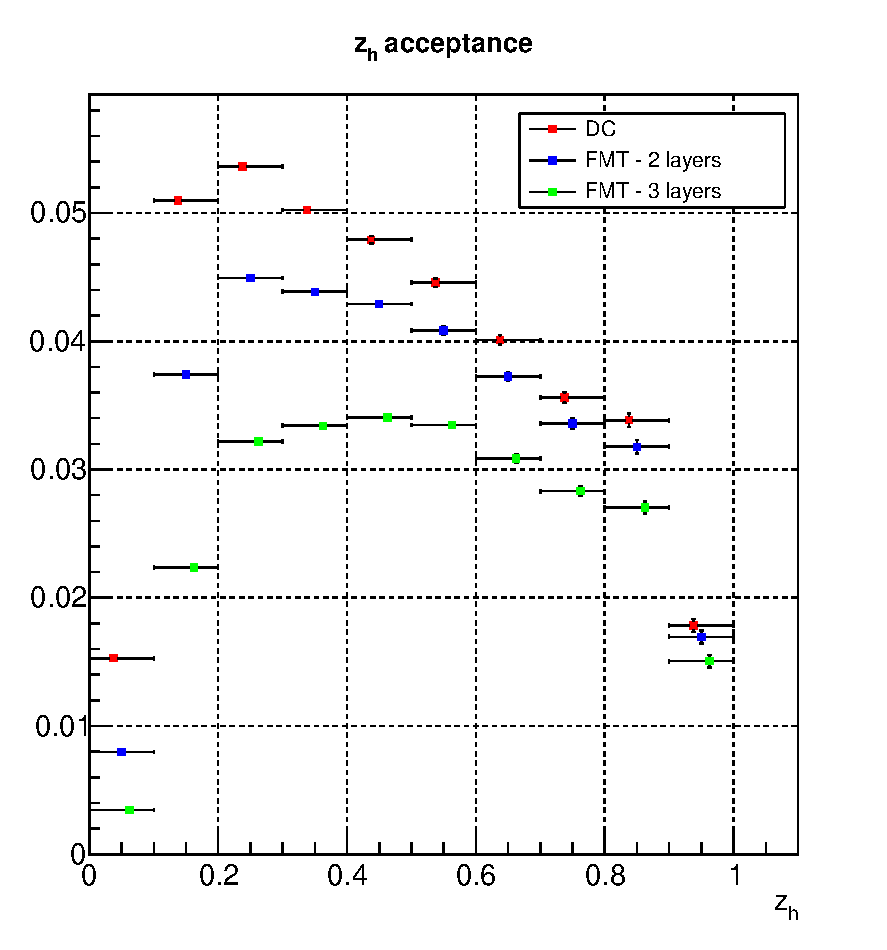
\includegraphics[width=\textwidth]{22zh_acc_211.pdf}
            \caption{$z_h$ acceptance for $e^-\pi^+$.}
            \label{fig::14.22::zh_acc_211}
        \end{subfigure}
        \hfill
        % pi-.
        \begin{subfigure}[b]{0.49\textwidth}
            \centering
            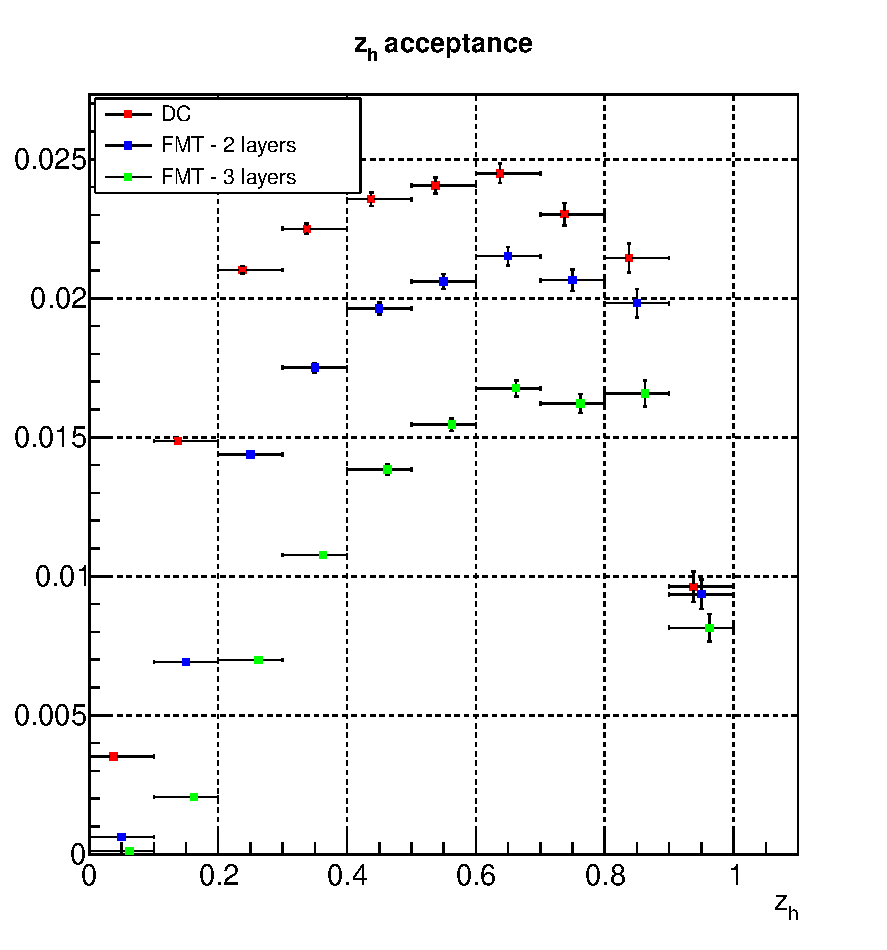
\includegraphics[width=\textwidth]{22zh_acc_-211.pdf}
            \caption{$z_h$ acceptance for $e^-\pi^-$.}
            \label{fig::14.22::zh_acc_-211}
        \end{subfigure}
        \caption[$z_h$ acceptance.]{$z_h$ acceptance for $e^-\pi^+$ and $e^-\pi^-$.
        All electron and other hadronic variables are integrated in both plots.
        The bin markers are slightly shifted in $x$ to improve legibility.
        Source: Own elaboration, using the \href{https://github.com/bleaktwig/clas12-rge-analysis}{clas12-rge-analysis} software.}
        \label{fig::14.22::zh_acc}
    \end{figure}

    % Pt2.
    \begin{figure}
        \centering
        % pi+.
        \begin{subfigure}[b]{0.49\textwidth}
            \centering
            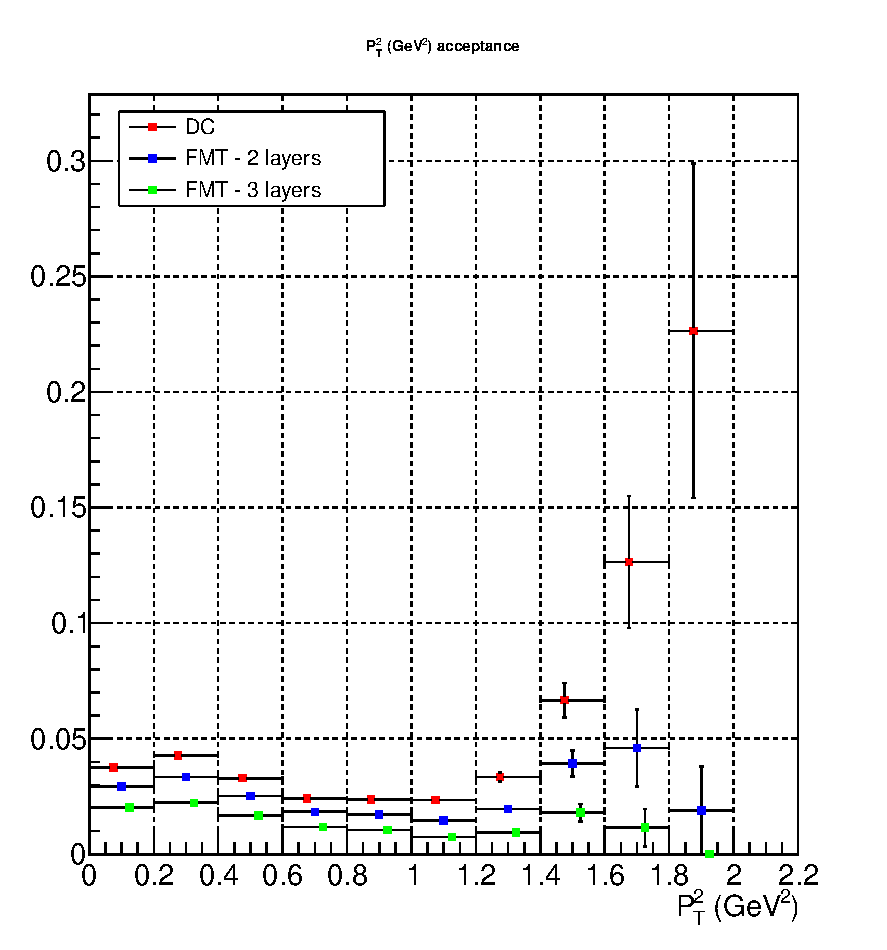
\includegraphics[width=\textwidth]{22pt2_acc_211.pdf}
            \caption{$p_T^2$ acceptance for $e^-\pi^+$.}
            \label{fig::14.22::pt2_acc_211}
        \end{subfigure}
        \hfill
        % pi-.
        \begin{subfigure}[b]{0.49\textwidth}
            \centering
            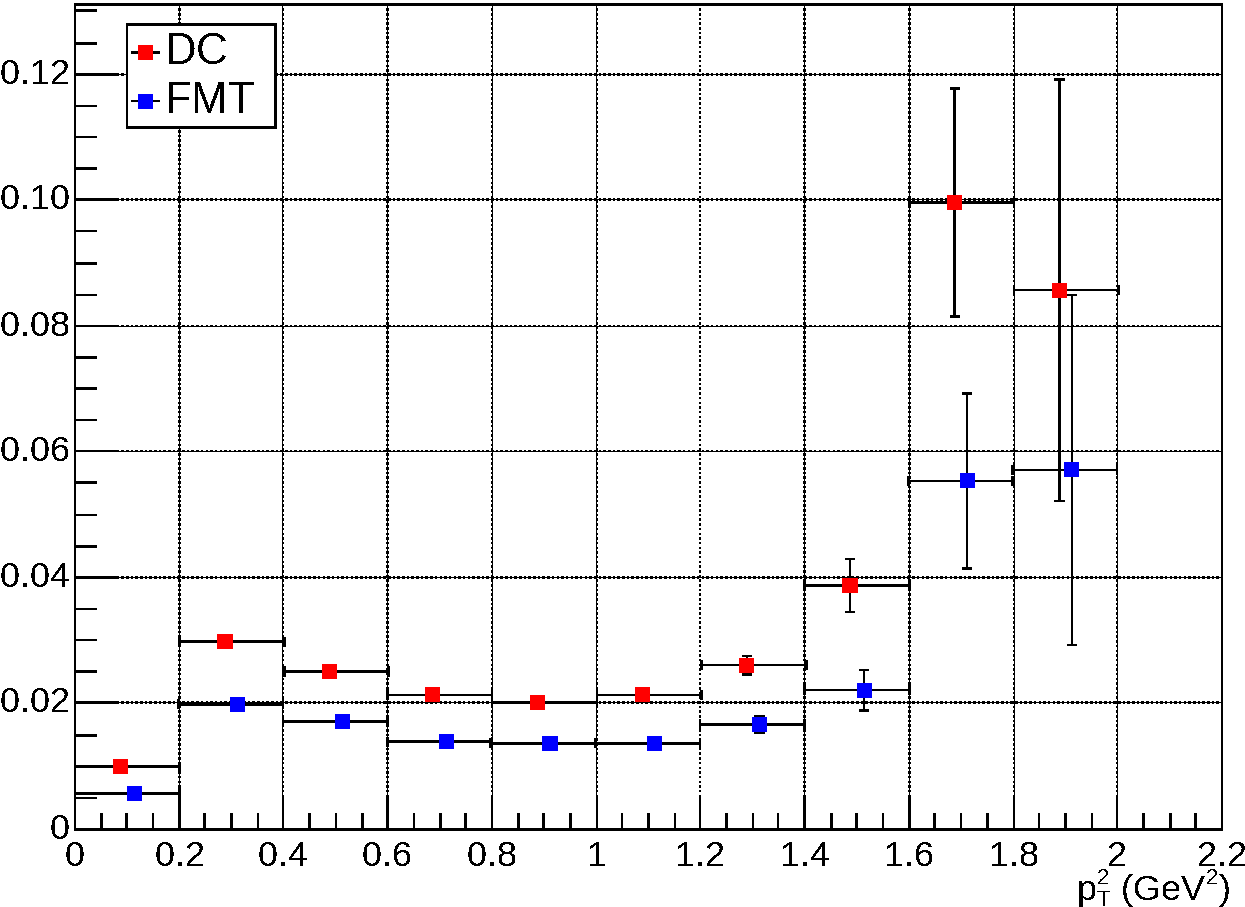
\includegraphics[width=\textwidth]{22pt2_acc_-211.pdf}
            \caption{$p_T^2$ acceptance for $e^-\pi^-$.}
            \label{fig::14.22::pt2_acc_-211}
        \end{subfigure}
        \caption[$p_T^2$ acceptance.]{$p_T^2$ acceptance for $e^-\pi^+$ and $e^-\pi^-$.
        All electron and other hadronic variables are integrated in both plots.
        The bin markers are slightly shifted in $x$ to improve legibility.
        Source: Own elaboration, using the \href{https://github.com/bleaktwig/clas12-rge-analysis}{clas12-rge-analysis} software.}
        \label{fig::14.22::pt2_acc}
    \end{figure}

    % phipq.
    \begin{figure}
        \centering
        % pi+.
        \begin{subfigure}[b]{0.49\textwidth}
            \centering
            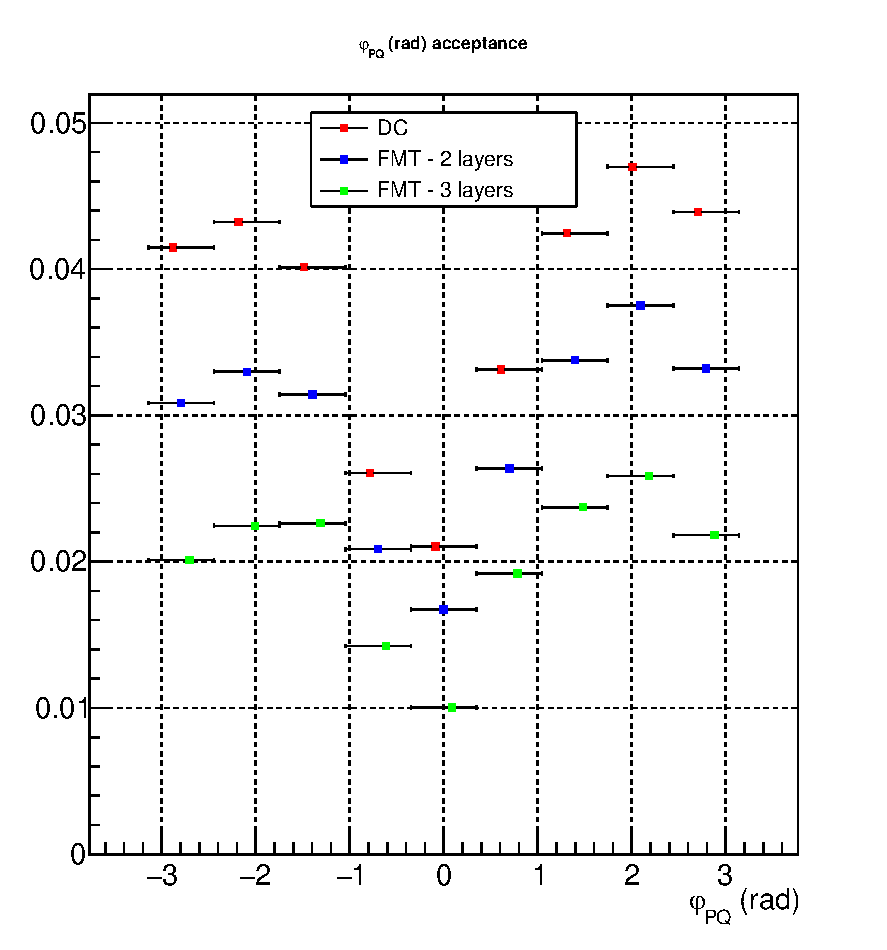
\includegraphics[width=\textwidth]{22phipq_acc_211.pdf}
            \caption{$\phi_{PQ}$ acceptance for $e^-\pi^+$.}
            \label{fig::14.22::phipq_acc_211}
        \end{subfigure}
        \hfill
        % pi-.
        \begin{subfigure}[b]{0.49\textwidth}
            \centering
            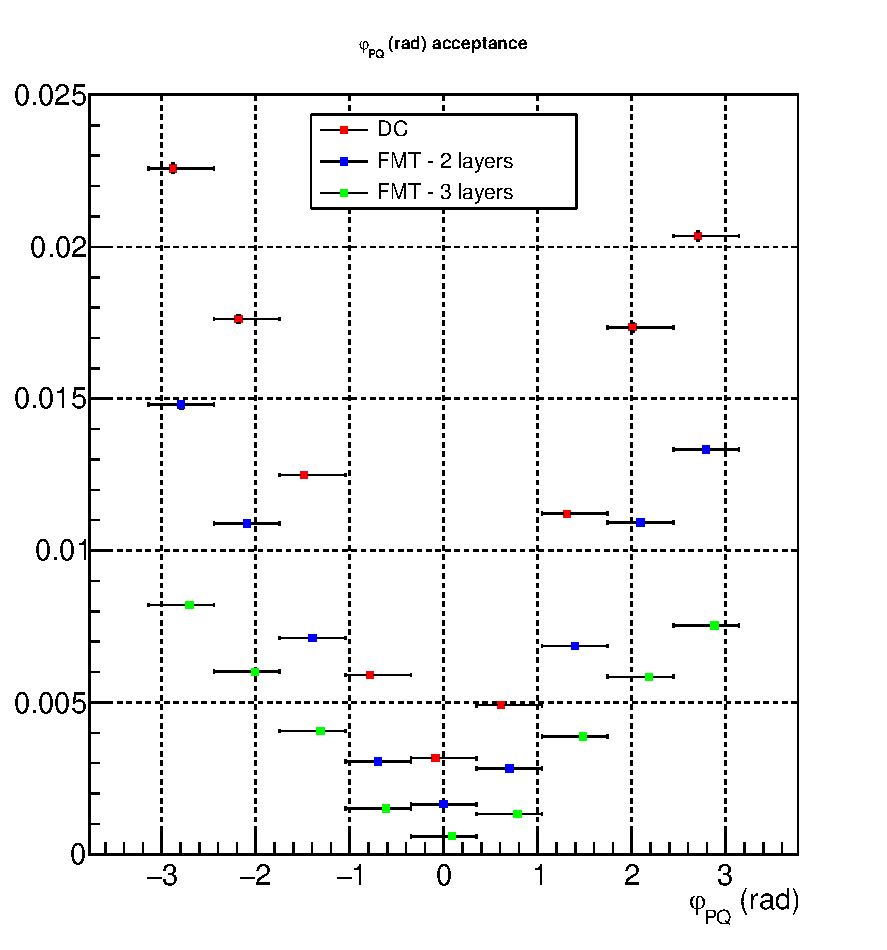
\includegraphics[width=\textwidth]{22phipq_acc_-211.pdf}
            \caption{$\phi_{PQ}$ acceptance for $e^-\pi^-$.}
            \label{fig::14.22::phipq_acc_-211}
        \end{subfigure}
        \caption[$\phi_{PQ}$ acceptance.]{$\phi_{PQ}$ acceptance for $e^-\pi^+$ and $e^-\pi^-$.
        All electron and other hadronic variables are integrated in both plots.
        The bin markers are slightly shifted in $x$ to improve legibility.
        Source: Own elaboration, using the \href{https://github.com/bleaktwig/clas12-rge-analysis}{clas12-rge-analysis} software.}
        \label{fig::14.22::phipq_acc}
    \end{figure}
